% !TEX TS-program = pdflatex
\documentclass[11pt]{article}

% -------------------- Packages --------------------
\usepackage[a4paper,margin=1in]{geometry}
\usepackage{amsmath,amssymb}
\usepackage[T1]{fontenc}
\usepackage{lmodern}
\usepackage{xcolor}
\usepackage{tcolorbox}
\tcbuselibrary{skins,breakable}
\usepackage{enumitem}
\usepackage{hyperref}
\usepackage{tikz}
\usetikzlibrary{calc,angles,quotes}

\pagestyle{empty}

% -------------------- Dark Theme Colors --------------------
\definecolor{bg}{HTML}{000000}
\definecolor{pairbg}{HTML}{121212}
\definecolor{solbg}{HTML}{0A0A0A}
\definecolor{border}{HTML}{2A2A2A}
\definecolor{text}{HTML}{FFFFFF}
\definecolor{muted}{HTML}{C9CDD3}
\definecolor{gold}{HTML}{FFD700}
\definecolor{green}{HTML}{4ADE80}
\definecolor{cyan}{HTML}{38BDF8}

\pagecolor{bg}
\color{text}

\hypersetup{
  colorlinks=true,
  linkcolor=cyan,
  urlcolor=cyan
}

\setlength{\parindent}{0pt}
\setlength{\parskip}{10pt}

\setlist[itemize]{left=1.4em,itemsep=6pt,topsep=6pt}
\setlist[enumerate]{left=1.6em,itemsep=4pt,topsep=4pt}

% (Optional safety net for rare overfull lines)
\setlength{\emergencystretch}{2em}

% -------------------- tcolorbox Base --------------------
\tcbset{
  enhanced,
  breakable,
  arc=12pt,
  boxrule=0.8pt,
  left=16pt,right=16pt,top=12pt,bottom=12pt
}

\newtcolorbox{QAPair}[1]{%
  colback=pairbg,
  colbacklower=solbg,
  colframe=border,
  coltext=text,
  title=\textcolor{gold}{\bfseries #1},
  fonttitle=\bfseries,
  coltitle=text,
  segmentation style={draw=border, dashed, line width=0.6pt},
}

% Visible text inside this box (fix)
\newtcolorbox{QuickBox}{%
  colback=pairbg,
  colframe=cyan,
  coltext=text,
  fontupper=\color{text},
  borderline north={4pt}{0pt}{cyan},
  arc=14pt,
  boxrule=0.8pt
}

% NEW: Small answer box for each sub-part (prevents overflow)
\newtcolorbox{SubAnsBox}[1]{%
  colback=solbg,
  colframe=border,
  coltext=text,
  title=\textcolor{cyan}{\bfseries #1},
  fonttitle=\bfseries,
  coltitle=text,
  arc=12pt,
  boxrule=0.7pt,
  left=12pt,right=12pt,top=8pt,bottom=8pt,
  breakable
}

% Helper for step headings
\newcommand{\Step}[1]{\textcolor{muted}{\textbf{Step #1:}}}

% Helper: multiline boxed answer that never overflows (used elsewhere)
\newcommand{\BoxAligned}[1]{%
\[
\boxed{\begin{aligned}
#1
\end{aligned}}
\]
}

% ============================================================
\begin{document}

\begin{center}
{\LARGE\bfseries \textcolor{gold}{Exercise 8.1 --- Solutions}}\\[-2pt]
\end{center}

\begin{QuickBox}
{\color{cyan}\bfseries Quick formulas (reference angles)}\par\medskip
\begin{itemize}
\item \textbf{Quadrant II (degrees):} if $90^\circ<\theta<180^\circ$, then reference angle $\theta_r=180^\circ-\theta$.
\item \textbf{Quadrant II (radians):} if $\frac{\pi}{2}<\theta<\pi$, then $\theta_r=\pi-\theta$.
\item \textbf{Supplement identities:}
\[
\sin(180^\circ-\theta)=\sin\theta,\quad
\cos(180^\circ-\theta)=-\cos\theta,\quad
\tan(180^\circ-\theta)=-\tan\theta.
\]
Equivalently,
\[
\sin(\pi-\theta)=\sin\theta,\quad
\cos(\pi-\theta)=-\cos\theta,\quad
\tan(\pi-\theta)=-\tan\theta.
\]
\end{itemize}
\end{QuickBox}

% ============================================================
% Q1
\begin{QAPair}{Question 1}
\textcolor{gold}{\bfseries Question:} Find the reference angles of: (i) $125^\circ$ \; (ii) $138^\circ$ \; (iii) $111^\circ$ \; (iv) $142^\circ$.\\
\tcblower
\textcolor{green}{\bfseries Answer:}

All given angles lie in \textbf{Quadrant II} (between $90^\circ$ and $180^\circ$), so
\[
\theta_r = 180^\circ-\theta.
\]

\[
\begin{aligned}
\text{(i)}\;& \theta=125^\circ \Rightarrow \theta_r=180^\circ-125^\circ=55^\circ.\\
\text{(ii)}\;& \theta=138^\circ \Rightarrow \theta_r=180^\circ-138^\circ=42^\circ.\\
\text{(iii)}\;& \theta=111^\circ \Rightarrow \theta_r=180^\circ-111^\circ=69^\circ.\\
\text{(iv)}\;& \theta=142^\circ \Rightarrow \theta_r=180^\circ-142^\circ=38^\circ.
\end{aligned}
\]

\medskip
\textcolor{muted}{(Diagram idea for Quadrant II reference angle)}\par
\begin{center}
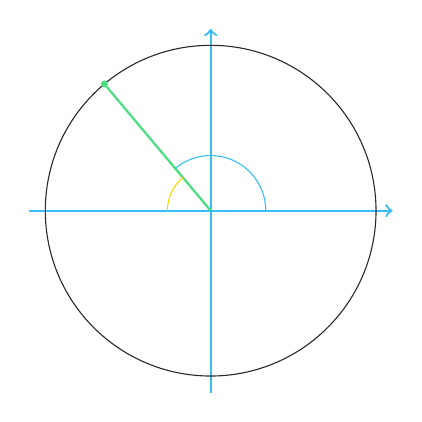
\begin{tikzpicture}[scale=1.05]
  \draw[->, thick, color=cyan] (-2.2,0) -- (2.2,0);
  \draw[->, thick, color=cyan] (0,-2.2) -- (0,2.2);
  \draw[color=border] (0,0) circle (2);
  \coordinate (A) at (2,0);
  \coordinate (B) at (0,0);
  \coordinate (P) at (130:2);
  \coordinate (N) at (-2,0);
  \draw[thick, color=green] (0,0) -- (P);
  \pic[draw=cyan, angle radius=0.7cm, angle eccentricity=1.25] {angle=A--B--P};
  \node[color=text] at (0.85,0.35) {$\theta$};
  \pic[draw=gold, angle radius=0.55cm, angle eccentricity=1.25] {angle=P--B--N};
  \node[color=text] at (-0.75,0.55) {$\theta_r$};
  \fill[color=green] (P) circle (1.2pt);
\end{tikzpicture}
\end{center}
\end{QAPair}

% ============================================================
% Q2
\begin{QAPair}{Question 2}
\textcolor{gold}{\bfseries Question:} If $\theta=36^\circ$, find equivalent angle $\alpha$ in the second quadrant for which $\sin\alpha=\sin\theta$.\\
\tcblower
\textcolor{green}{\bfseries Answer:}
\[
\Step{1}\; \text{In Quadrant II, } \sin(180^\circ-\theta)=\sin\theta.
\]
\[
\Step{2}\; \alpha=180^\circ-\theta=180^\circ-36^\circ=144^\circ.
\]
\[
\boxed{\alpha=144^\circ}
\]
\end{QAPair}

% ============================================================
% Q3
\begin{QAPair}{Question 3}
\textcolor{gold}{\bfseries Question:} If $\theta=87^\circ$, find equivalent angle $\beta$ in the second quadrant for which $\cos\beta=-\cos\theta$.\\
\tcblower
\textcolor{green}{\bfseries Answer:}
\[
\Step{1}\; \cos(180^\circ-\theta)=-\cos\theta.
\]
\[
\Step{2}\; \beta=180^\circ-\theta=180^\circ-87^\circ=93^\circ.
\]
\[
\boxed{\beta=93^\circ}
\]
\end{QAPair}

% ============================================================
% Q4
\begin{QAPair}{Question 4}
\textcolor{gold}{\bfseries Question:} Using a reference angle, find the exact values of $\sin120^\circ$, $\cos120^\circ$ and $\tan120^\circ$.\\
\tcblower
\textcolor{green}{\bfseries Answer:}
\[
\Step{1}\; 120^\circ \text{ is in Quadrant II, so } \theta_r=180^\circ-120^\circ=60^\circ.
\]
\[
\Step{2}\; \sin120^\circ=\sin60^\circ=\frac{\sqrt3}{2} \quad (\text{sine is + in QII})
\]
\[
\Step{3}\; \cos120^\circ=-\cos60^\circ=-\frac12 \quad (\text{cosine is -- in QII})
\]
\[
\Step{4}\; \tan120^\circ=\frac{\sin120^\circ}{\cos120^\circ}
=\frac{\frac{\sqrt3}{2}}{-\frac12}=-\sqrt3.
\]

\[
\boxed{\sin120^\circ=\frac{\sqrt3}{2},\;\;\cos120^\circ=-\frac12,\;\;\tan120^\circ=-\sqrt3}
\]
\end{QAPair}

% ============================================================
% Q5
\begin{QAPair}{Question 5}
\textcolor{gold}{\bfseries Question:} Using the reference angle, find $\cos\frac{3\pi}{4}$, $\sin\frac{3\pi}{4}$ and $\tan\frac{3\pi}{4}$.\\
\tcblower
\textcolor{green}{\bfseries Answer:}
\[
\Step{1}\; \frac{3\pi}{4}=135^\circ \text{ lies in Quadrant II.}
\]
\[
\Step{2}\; \theta_r=\pi-\frac{3\pi}{4}=\frac{\pi}{4}.
\]
\BoxAligned{
\cos\frac{3\pi}{4} &= -\frac{\sqrt2}{2},\\
\sin\frac{3\pi}{4} &= \frac{\sqrt2}{2},\\
\tan\frac{3\pi}{4} &= -1.
}
\end{QAPair}

% ============================================================
% Q6 (FIXED: no overflow + separate boxes for each sub-part)
\begin{QAPair}{Question 6}
\textcolor{gold}{\bfseries Question:} If $\cos\theta=0.559$, find: \\
(i) $\cos(180^\circ-\theta)$ \quad
(ii) $\sin(180^\circ-\theta)$ \quad
(iii) $\tan(180^\circ-\theta)$ \\
(iv) $\cot(180^\circ-\theta)$ \quad
(v) $\sec(180^\circ-\theta)$ \quad
(vi) $\cosec(180^\circ-\theta)$.\\
\tcblower
\textcolor{green}{\bfseries Answer:}

\textcolor{muted}{Since $\cos\theta>0$, we take $\theta$ as acute (Quadrant I), so $\sin\theta>0$. Then $180^\circ-\theta$ lies in Quadrant II.}
\[
\Step{1}\; \text{Calculate } \sin\theta
\]
\[
\begin{aligned}
\sin\theta
&=\sqrt{1-\cos^2\theta}\\
&=\sqrt{1-(0.559)^2}\\
&=\sqrt{1-0.312481}\\
&=\sqrt{0.687519}\\
&\approx 0.829.
\end{aligned}
\]


\[
\Step{2}\; \text{Use supplement identities }
\]
\[
\cos(180^\circ-\theta)=-\cos\theta,
\]
\[
\sin(180^\circ-\theta)=\sin\theta,
\]
\[
\tan(180^\circ-\theta)=-\tan\theta.
\]


First compute (for reference):
\[
\begin{aligned}
\tan\theta &= \frac{\sin\theta}{\cos\theta}\approx \frac{0.829}{0.559}\approx 1.483,\\
\sec\theta &= \frac{1}{\cos\theta}\approx \frac{1}{0.559}\approx 1.789,\\
\cosec\theta &= \frac{1}{\sin\theta}\approx \frac{1}{0.829}\approx 1.206.
\end{aligned}
\]

\medskip

\begin{SubAnsBox}{(i) $\;\cos(180^\circ-\theta)$}
\[
\cos(180^\circ-\theta)=-\cos\theta=-0.559
\]
\end{SubAnsBox}

\begin{SubAnsBox}{(ii) $\;\sin(180^\circ-\theta)$}
\[
\sin(180^\circ-\theta)=\sin\theta\approx 0.829
\]
\end{SubAnsBox}

\begin{SubAnsBox}{(iii) $\;\tan(180^\circ-\theta)$}
\[
\tan(180^\circ-\theta)=-\tan\theta\approx -1.483
\]
\end{SubAnsBox}

\begin{SubAnsBox}{(iv) $\;\cot(180^\circ-\theta)$}
\[
\cot(180^\circ-\theta)=-\cot\theta
=-\frac{1}{\tan\theta}\approx -0.674
\]
\end{SubAnsBox}

\begin{SubAnsBox}{(v) $\;\sec(180^\circ-\theta)$}
\[
\sec(180^\circ-\theta)=-\sec\theta\approx -1.789
\]
\end{SubAnsBox}

\begin{SubAnsBox}{(vi) $\;\cosec(180^\circ-\theta)$}
\[
\cosec(180^\circ-\theta)=\cosec\theta\approx 1.206
\]
\end{SubAnsBox}

\end{QAPair}

\end{document}
